\documentclass{beamer}

\usetheme{Madrid}
\setbeamertemplate{navigation symbols}{} 
\setbeamertemplate{itemize items}[default]
\definecolor{unifiBlue}{HTML}{004180}
\definecolor{unifiRed}{HTML}{E0000D}
\usecolortheme[named=unifiBlue]{structure}

\AtBeginSection[]{
	\begin{frame}
		\vfill
		\centering
		\begin{beamercolorbox}[sep=8pt,center,shadow=true,rounded=true]{title}
			\usebeamerfont{title}\secname\par
		\end{beamercolorbox}
		\vfill
	\end{frame}
}

\usepackage[utf8]{inputenc}
\usepackage{graphicx} 
\usepackage{mathtools}
\usepackage{multirow}
\usepackage{lmodern}
\usepackage{xparse}	
\usepackage{arydshln}

\graphicspath{{images/}}

\newcommand{\defeq}{\vcentcolon=}
\newcommand{\eqdef}{=\vcentcolon}
\newcommand{\pushone}{\texttt{\textsc{push}}\textsubscript{\texttt{1}}}
\newcommand{\pushzero}{\texttt{\textsc{push}}\textsubscript{\texttt{0}}}
\newcommand{\nonempty}{\textsc{\texttt{nonempty}}}
\newcommand{\tos}{\textsc{\texttt{top}}}
\newcommand{\pop}{\textsc{\texttt{pop}}}
\newcommand{\noop}{\textsc{\texttt{noop}}}
\newcommand{\Q}{\mathbb{Q}}
\newcommand{\h}{_\text{h}}
\newcommand{\shortTos}{\textsc{\texttt{t}}}
\newcommand{\shortNonempty}{\textsc{\texttt{ne}}}
\renewcommand{\arraystretch}{1.3}
\NewDocumentCommand{\overarrow}{O{=} O{\uparrow} m}{%
	\overset{\makebox[0pt]{\begin{tabular}{@{}c@{}}#3\\[0pt]\ensuremath{#2}\end{tabular}}}{#1}
}

\title[Turing Completeness of RNNs]{On the Turing Completeness of Recurrent Neural Networks} 
\author{Francesco Ballerini} 
\institute[]
{
Università degli Studi di Firenze\\ 
Scuola di Ingegneria 
}
\date{February 27th 2020} 

\begin{document}

{
	\usebackgroundtemplate{
		\begin{picture}(0,595)
			\hspace*{3cm}
			
\includegraphics[scale=1.5]{banner.pdf}
		\end{picture}
	}
	\begin{frame}
		\titlepage 
	\end{frame}
}

\section{Motivations}

\begin{frame}{Why neural networks}
	\textcolor{unifiRed}{Deep learning} (deep neural networks) is currently the prevalent machine-learning approach for:
	\begin{itemize}
		\pause
		\item Computer vision
		\pause
		\item Natural-language processing
		\pause
		\item In general, all perceptual tasks
	\end{itemize}
\end{frame}

\begin{frame}{Why Turing completeness}	
	From a theory-of-computation standpoint:
	\begin{itemize}
		\pause 
		\item It would be nice to know that neural networks are as powerful as Turing machines (TMs)
		\pause
		\item So as to ensure that any \textcolor{unifiRed}{effectively calculable} function is computable by a neural network (Church--Turing thesis)
	\end{itemize}
\end{frame}

\begin{frame}{The result}
	\only<1>{As it turns out, given a TM, we can build a \textcolor{unifiRed}{recurrent} neural network (RNN) with \textcolor{unifiRed}{rational weights and biases} that computes the same function as the TM}
	\only<2->{
		This result bridges two worlds:
		\begin{itemize}
			\item<3-> \textcolor{unifiRed}{Symbolic} computation (TMs):
			\begin{itemize}
				\item<4-> Finite alphabets of symbols
				\item<5-> Explicit separation of control (state) and memory (tape)
				\item<6> If--then conditionals used for updates
			\end{itemize}
			\item<3-> ``\textcolor{unifiRed}{Neural}'' computation (RNNs):
			\begin{itemize}
				\item<4-> Continuous values
				\item<5-> No intrinsic separation of state vs memory
				\item<6> No intrinsic Boolean logic
			\end{itemize}
		\end{itemize}
	}
	
\end{frame}

\section{Our contribution}

\begin{frame}{The original article}
	\begin{itemize}
		\item The original proof is contained in an article named ``On the Computational Power of Neural Nets'' by \textcolor{unifiRed}{Hava Siegelmann} and \textcolor{unifiRed}{Eduardo Sontag}
		\pause
		\item The article dates back to \textcolor{unifiRed}{1992}
	\end{itemize}
\end{frame}

\begin{frame}{Our modernization}
	What we did was:
	\begin{itemize}
		\pause
		\item Updating the formalism and terminology according to what is widely used today
		\pause
		\item Adding 
		\begin{itemize}
			\pause
			\item Figures
			\pause 
			\item Tables
			\pause
			\item Explicit calculations
			\pause
		\end{itemize}
		in order to leave as little as possible to the imagination of the reader
		\pause
		\item Adding an example in which we apply the construction showed in the proof
		\begin{itemize}
			\pause
			\item And providing a Python implementation of such example
			\pause
		\end{itemize}
		\item Most importantly, giving a more detailed and (hopefully) pleasant structure to the proof itself
		\begin{itemize}
			\pause
			\item Which, in our experience, was pretty frustrating to make sense of
		\end{itemize}
	\end{itemize}
\end{frame}

\section{Preliminaries}

\begin{frame}{What this presentation is about}
	\begin{itemize}
		\item We will not show the formal proof of the general case
		\pause		
		\item Instead, we will focus on an example of how to build an RNN that simulates a TM
		\pause
		\item And, actually, instead of considering a TM, we will start from a \textcolor{unifiRed}{double-stack pushdown automaton} (double-stack PDA)
		\pause
		\item This is not a problem, since double-stack PDAs can be proven to be computationally equivalent to single-tape TMs
		\begin{itemize}
			\pause
			\item That is, a function is computable by a double-stack PDA if and only if it is computable by a single-tape TM
		\end{itemize}
	\end{itemize}
\end{frame}

\begin{frame}{Rational stack encoding}
	\begin{itemize}
		\item We want to encode a stack content as a number 
		\pause
		\begin{itemize}
			\item This will turn out to be useful later \dots
			\pause
		\end{itemize}
		\item We will work with PDAs with two \textcolor{unifiRed}{binary} stacks
		\pause
		\begin{itemize}
			\item Equivalent to \textcolor{unifiRed}{binary} single-tape TMs
			\pause
		\end{itemize}
		\item We choose the following encoding, where $a_i\in\{0,1\}$:
		\begin{table}
			\centering
			\begin{tabular}{|c| c}
				\cline{1-1}
				$a_1$   &\multirow{4}{*}{$\,\longrightarrow\;\,\displaystyle{q=\sum_{i=1}^{n}\frac{2a_i+1}{4^i}\in\Q}$}\\
				\cline{1-1}
				$a_2$   &\\
				\cline{1-1}
				$\vdots$&\\
				\cline{1-1}
				$a_n$   &\\
				\cline{1-1}
			\end{tabular}
		\end{table}
		\pause
		\item $q\in[0,1)$
		\pause
		\begin{itemize}
			\item So, it might be a good candidate for a neuron activation \dots
		\end{itemize}
	\end{itemize}
\end{frame}

\section{PDA $\to$ RNN}

\begin{frame}[b]{Double-stack PDA computing unary addition}
	\only<1-4>{
		\begin{figure}
			\centering
			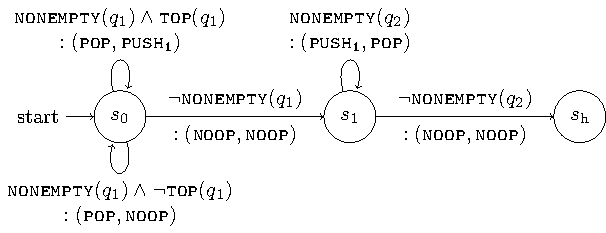
\includegraphics{PDA.pdf}
		\end{figure}
		\begin{itemize}
			\pause
			\item Stack 1 starts with the two unary numbers to add separated by a zero
			\pause
			\item Stack 2 starts empty
			\begin{itemize}
				\pause
				\item E.g.
				\begin{tabular}{c c c c}
					\cline{2-2}
					\multirow{3}{*}{$1+1\longrightarrow$}&\multicolumn{1}{|c|}{1}&&\\
					\cline{2-2}
					                                     &\multicolumn{1}{|c|}{0}&&\\
					\cline{2-2}\cline{4-4}
					                                     &\multicolumn{1}{|c|}{1}&&\multicolumn{1}{|c|}{$\varepsilon$}\\
					\cline{2-2}\cline{4-4}
				\end{tabular}
			\end{itemize}
		\end{itemize}
	}
	\only<5>{
		\begin{table}
			\begin{tabular}{c c c}
				\multicolumn{3}{c}{\textcolor{unifiRed}{Start}}\\\vspace{-5mm}
				&&\\
				\cline{1-1}
				\multicolumn{1}{|c|}{1}&&\\
				\cline{1-1}
				\multicolumn{1}{|c|}{0}&&\\
				\cline{1-1}\cline{3-3}
				\multicolumn{1}{|c|}{1}&&\multicolumn{1}{|c|}{$\varepsilon$}\\
				\cline{1-1}\cline{3-3}
			\end{tabular}
		\end{table}
		\vspace{3.2cm}
	}
	\only<6>{
		\begin{table}
			\begin{tabular}{c c c}
				\cline{1-1}
				\multicolumn{1}{|c|}{0}&&\\
				\cline{1-1}\cline{3-3}
				\multicolumn{1}{|c|}{1}&&\multicolumn{1}{|c|}{1}\\
				\cline{1-1}\cline{3-3}
			\end{tabular}
		\end{table}
		\vspace{3.2cm}
	}
	\only<7>{
		\begin{table}
			\begin{tabular}{c c c}
				\cline{1-1}\cline{3-3}
				\multicolumn{1}{|c|}{1}&&\multicolumn{1}{|c|}{1}\\
				\cline{1-1}\cline{3-3}
			\end{tabular}
		\end{table}
		\vspace{3.2cm}
	}
	\only<8>{
		\begin{table}
			\begin{tabular}{c c c}
				\cline{3-3}
				&&\multicolumn{1}{|c|}{1}\\
				\cline{1-1}\cline{3-3}
				\multicolumn{1}{|c|}{$\varepsilon$}&&\multicolumn{1}{|c|}{1}\\
				\cline{1-1}\cline{3-3}
			\end{tabular}
		\end{table}
		\vspace{3.2cm}
	}
	\only<9>{
		\begin{table}
			\begin{tabular}{c c c}
				\cline{1-1}\cline{3-3}
				\multicolumn{1}{|c|}{1}&&\multicolumn{1}{|c|}{1}\\
				\cline{1-1}\cline{3-3}
			\end{tabular}
		\end{table}
		\vspace{3.2cm}
	}
	\only<10>{
		\begin{table}
			\begin{tabular}{c c c}
				\multicolumn{3}{c}{\textcolor{unifiRed}{Halt}}\\\vspace{-5mm}
				&&\\
				\cline{1-1}
				\multicolumn{1}{|c|}{1}&&\\
				\cline{1-1}\cline{3-3}
				\multicolumn{1}{|c|}{1}&&\multicolumn{1}{|c|}{$\varepsilon$}\\
				\cline{1-1}\cline{3-3}
			\end{tabular}
		\end{table}
		\vspace{3.2cm}
	}
\end{frame}

\begin{frame}{Defining the neural-network input layer}
	\begin{itemize}
		\item At a given time $t$, the PDA is uniquely described by
		\begin{itemize}
			\pause
			\item Its state
			\pause
			\item The content of stack 1
			\pause
			\item The content of stack 2
		\end{itemize}
		\pause
		\item We want to be able to express the description of the PDA at time $t$ as a neural-network layer
		\pause
		\item To do so, consider the tuple $(x_0,x_1,x\h,q_1,q_2)\in\Q^5$, where:
		\begin{itemize}
			\pause
			\item
			$
				(x_0,x_1,x\h)= 
					\begin{cases}
						(1,0,0)&\text{if the PDA is in state }s_0\\\pause
						(0,1,0)&\text{if the PDA is in state }s_1\\\pause
						(0,0,1)&\text{if the PDA is in state }s\h
					\end{cases}
			$
			\pause
			\item $q_{1,2}\in[0,1)$ is the rational encoding of the content of stack $1,2$
		\end{itemize}	
		\pause
		\item Therefore, $(x_0,x_1,x\h,q_1,q_2)$ will be the \textcolor{unifiRed}{input layer} of the neural network we are building
	\end{itemize}
\end{frame}

\begin{frame}{Defining the neural-network output layer}
	\begin{itemize}
		\item Let $(x_0^+,x_1^+,x\h^+,q_1^+,q_2^+)$ be the description of the PDA at time $t+1$	
		\pause
		\item We would like $(x_0^+,x_1^+,x\h^+,q_1^+,q_2^+)$ to be the \textcolor{unifiRed}{output layer} of our network
		\pause
		\item Is it possible to go from input to output layer, that is $$(x_0,x_1,x\h,q_1,q_2)\longrightarrow(x_0^+,x_1^+,x\h^+,q_1^+,q_2^+)$$ using only neural-network operations?
		\pause
		\item Namely, something like $\sigma(Wa+b)$, where:
		\begin{itemize}
			\pause
			\item $\sigma$ is a \textcolor{unifiRed}{sigmoid function}
			\pause
			\item $W$ is a matrix
			\pause
			\item $a$ and $b$ are vectors
		\end{itemize}
	\end{itemize}
\end{frame}

\begin{frame}[t]{}
	\begin{itemize}
		\item Yes, it is!
		\pause 
		\item Let us start from $x_0^+$:
		\only<3>{
			\begin{align*}
				x_0^+=\textcolor{unifiRed}{\sigma(}x_0^+\textcolor{unifiRed}{)}\hspace{5.8cm}
			\end{align*}
			where $\sigma$ is 
				\begin{figure}
					\centering
					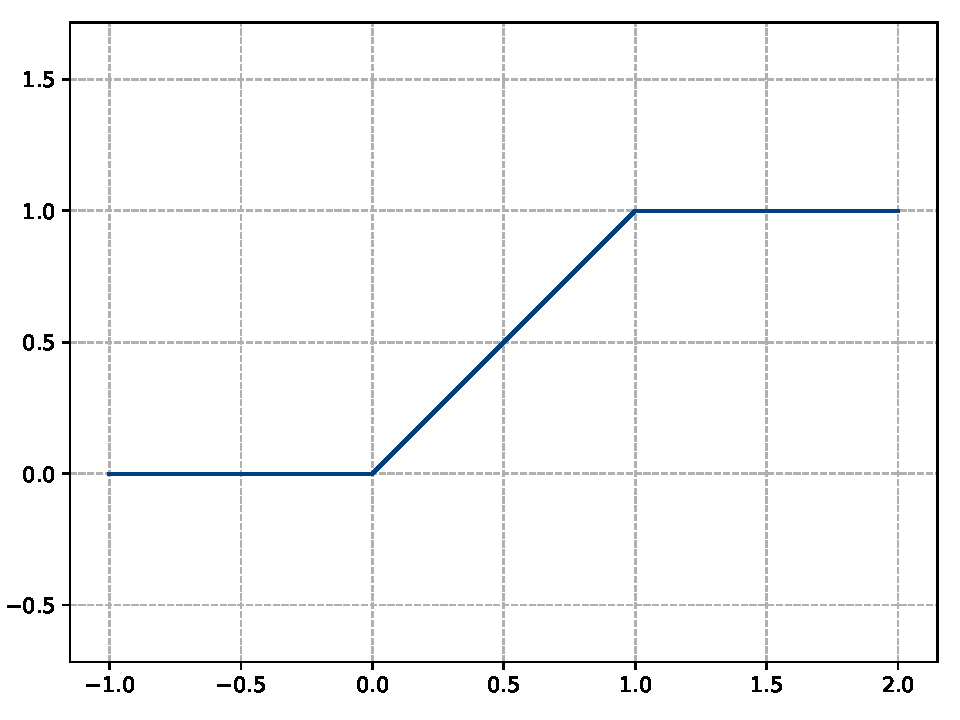
\includegraphics[scale=.35]{sigma.pdf}
				\end{figure}
				(remember that $x_0^+\in\{0,1\}$)
		}
		\only<4>{
			\begin{align*}
				x_0^+=\sigma(&x_0^+)\\
					 =\sigma(&\textcolor{unifiRed}{x_0\cdot\nonempty(q_1)\cdot\tos(q_1)\:+}\hspace{1.6cm}\\
							 &\textcolor{unifiRed}{x_0\cdot\nonempty(q_1)\cdot\lnot\tos(q_1)})
			\end{align*}
			since
			\begin{figure}
				\centering
				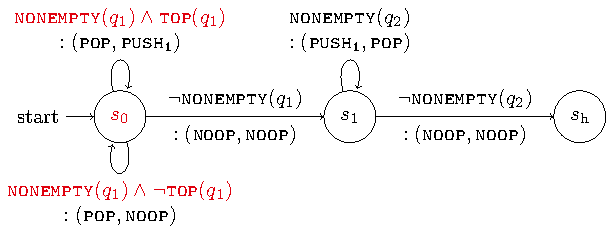
\includegraphics{redPDA.pdf}
			\end{figure}
		}
		\only<5>{
			\begin{align*}
				x_0^+=\sigma(&x_0^+)\\
					 =\sigma(&x_0\cdot\nonempty(q_1)\cdot\tos(q_1)\:+\\
							 &x_0\cdot\nonempty(q_1)\cdot\lnot\tos(q_1))\\	
					 =\sigma(&\textcolor{unifiRed}{\sigma(x_0+\nonempty(q_1)+\tos(q_1)-2)}\:+\\
							 &\textcolor{unifiRed}{\sigma(x_0+\nonempty(q_1)+\lnot\tos(q_1)-2)})
			\end{align*}
			because of the following lemma:
			\begin{lemma}
				Let $a_1,a_2,\dots,a_k\in\{0,1\}$. Then
				$$
					a_1a_2\dots a_k=\sigma(a_1+a_2+\dots+a_k-k+1)
				$$
			\end{lemma}
		}
		\only<6>{
			\begin{align*}
				x_0^+=\sigma(&x_0^+)\\
					 =\sigma(&x_0\cdot\nonempty(q_1)\cdot\tos(q_1)\:+\\
							 &x_0\cdot\nonempty(q_1)\cdot\lnot\tos(q_1))\\	
					 =\sigma(&\sigma(x_0+\nonempty(q_1)+\tos(q_1)-2)\:+\\
							 &\sigma(x_0+\nonempty(q_1)+\lnot\tos(q_1)-2))\\
					 =\sigma(&\sigma(x_0+\textcolor{unifiRed}{\sigma(4q_1)}+\textcolor{unifiRed}{\sigma(4q_1-2)}-2)\:+ \\
							 &\sigma(x_0+\textcolor{unifiRed}{\sigma(4q_1)}+\textcolor{unifiRed}{1-\sigma(q_1-2)}-2))
			\end{align*}
			because of the following theorem:\small
			\begin{theorem}
				Let $q$ be the rational encoding of a stack content. Then$$\tos(q)=\sigma(4q-2),\quad\nonempty(q)=\sigma(4q)$$
			\end{theorem}
			
		}
		\only<7>{
			\begin{align*}
				x_0^+=\sigma(&x_0^+)\\
					 =\sigma(&x_0\cdot\nonempty(q_1)\cdot\tos(q_1)\:+\\
							 &x_0\cdot\nonempty(q_1)\cdot\lnot\tos(q_1))\\	
					 =\sigma(&\sigma(x_0+\nonempty(q_1)+\tos(q_1)-2)\:+\\
							 &\sigma(x_0+\nonempty(q_1)+\lnot\tos(q_1)-2))\\
					 =\sigma(&\sigma(x_0+\sigma(4q_1)+\sigma(4q_1-2)-2)\:+ \\
							 &\sigma(x_0+\sigma(4q_1)-\sigma(q_1-2)\color{unifiRed}-1\color{black}))
			\end{align*}
		}
	\end{itemize}
\end{frame}

\begin{frame}{Input layer $\to$ output layer}
	\only<1-5>{
		\begin{itemize}
			\item We did it! We computed $x_0^+$ using only $\sigma$ and linear combinations of input-layer activations $(x_0,x_1,x\h,q_1,q_2)$
			\begin{itemize}
				\pause
				\item In particular, we used $x_0$ and $q_1$
			\end{itemize}
			\pause
			\item From the expression we got, though, we can see that we will not be able to go from $(x_0,x_1,x\h,q_1,q_2)$ to $x_0^+$ in just one step
			\pause
			\item Instead, we will need some \textcolor{unifiRed}{inner} (i.e. intermediate) \textcolor{unifiRed}{layers} $\ell_{1,2}$:
			\pause
		\end{itemize}
		\small
		\begin{align*}
			x_0^+=\underbrace{\sigma(
				\underbrace{\sigma(
					\overarrow[x_0]{\scriptsize input}+
					\underbrace{\sigma(4\overarrow[q_1]{\scriptsize input})}_\text{\scriptsize $\ell_1$}+
					\underbrace{\sigma(4\overarrow[q_1]{\scriptsize input}-2)}_\text{\scriptsize $\ell_1$}
					-2)
				}_\text{\scriptsize $\ell_2$}+
				\underbrace{\sigma(
					\overarrow[x_0]{\scriptsize input}+
					\underbrace{\sigma(4\overarrow[q_1]{\scriptsize input})}_\text{\scriptsize $\ell_1$}-
					\underbrace{\sigma(4\overarrow[q_1]{\scriptsize input}-2)}_\text{\scriptsize $\ell_1$}
					-1)
				}_\text{\scriptsize $\ell_2$})
			}_\text{\scriptsize output}
		\end{align*}
	}
	\only<6-11>{
		\begin{itemize}
			\item We can do the same for:
			\begin{align*}
			\onslide<7->{
				(x_0,x_1,x\h,q_1,q_2)&\longrightarrow x_1^+\\
			}
			\onslide<8->{
				(x_0,x_1,x\h,q_1,q_2)&\longrightarrow x\h^+\\
			}
			\onslide<9->{
				(x_0,x_1,x\h,q_1,q_2)&\longrightarrow q_1^+\\
			}
			\onslide<10->{
				(x_0,x_1,x\h,q_1,q_2)&\longrightarrow q_2^+
			}
			\end{align*}
			\onslide<11>{\item Let us skip the calculations (which are similar to those we have already seen anyway) and just show the final results:}
		\end{itemize}
	}
	\only<12-15>{
		\begin{align*}
		\onslide<12->{x_1^+=\dots=\sigma(&\sigma(x_0-\sigma(4q_1))+\sigma(x_1+\sigma(4q_2)-1))\\}
		\onslide<13->{x\h^+=\dots=\sigma(&\sigma(x_1-\sigma(4q_2)))\\}
		\onslide<14->{
			q_1^+=\dots=\sigma\big(&\sigma(x_0+\sigma(4q_1)-\sigma(4q_1-2)+4q_1-4)\:+\\
								   &\sigma(x_0+\sigma(4q_1)-3\sigma(4q_1-2)+4q_1-3)\:+\\
								   &\sigma(x_0-\sigma(4q_1)+q_1-1)\:+\\
								   &\sigma\big(x_1+\sigma(4q_2)+\textstyle{\frac{1}{4}}q_1-\textstyle{\frac{5}{4}}\big)\:+\\
								   &\sigma(x_1-\sigma(4q_2)+q_1-1)\big)\\
		}
		\onslide<15>{
			q_2^+=\dots=\sigma\big(&\sigma\big(x_0+\sigma(4q_1)-\sigma(4q_1-2)+\textstyle{\frac{1}{4}}q_2-\textstyle{\frac{9}{4}}\big)\:+\\
								   &\sigma(x_0+\sigma(4q_1)-\sigma(4q_1-2)+q_2-2)\:+\\
								   &\sigma(x_0-\sigma(4q_1)+q_2-1)\:+\\
								   &\sigma(x_1+\sigma(4q_2)-2\sigma(4q_2-2)+4q_2-3)\:+\\
								   &\sigma(x_1-\sigma(4q_2)+q_2-1)\big)
		}
		\end{align*}
	}
\end{frame}

\begin{frame}{The network}
	\begin{itemize}
		\item We are done: we built a neural network whose input layer is the description of the PDA at time $t$, namely, $$(x_0,x_1,x\h,q_1,q_2)$$ \pause and whose output layer is the description of the PDA at time $t+1$, that is, $$(x_0^+,x_1^+,x\h^+,q_1^+,q_2^+)$$
		\pause
		\item Let us look at its graphical depiction:
	\end{itemize}
\end{frame}

\begin{frame}[plain, noframenumbering]
	\begin{figure}
		\centering
		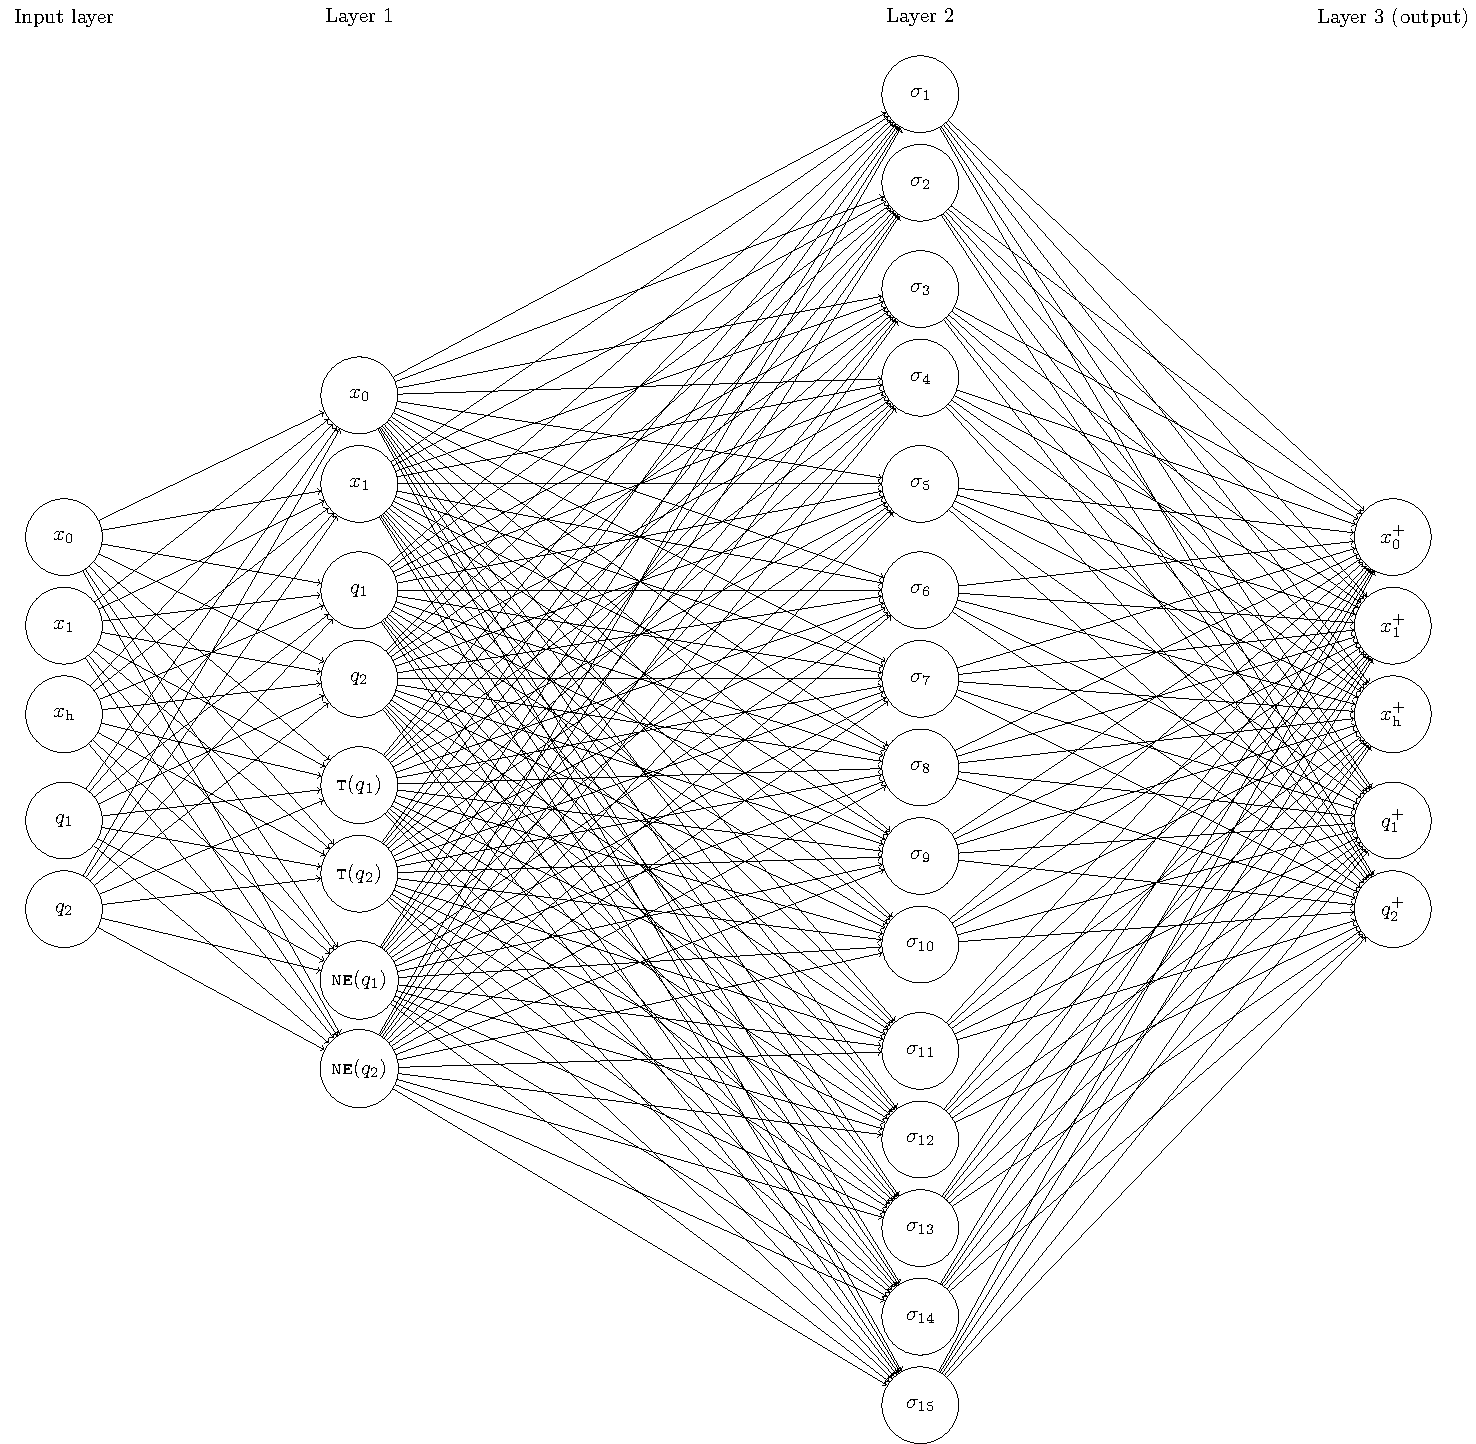
\includegraphics[scale=.38]{exampleNetSlides.pdf}
	\end{figure}
\end{frame}

\begin{frame}{Simulation}
	Now that we have built the network, how do we simulate a PDA execution with it?
	\onslide<2->{
		\begin{block}{Simulation algorithm}
			\begin{enumerate}
				\item Initialize the network with input layer $$(x_0,x_1,x\h,q_1,q_2)=(1,0,0,q_1,q_2)$$
				\onslide<3->{where $q_{1,2}$ is the rational encoding of the content of stack $1,2$ at the beginning of the PDA execution}
				\onslide<4->{\item Compute the output layer $(x_0^+,x_1^+,x\h^+,q_1^+,q_2^+)$ \label{itm:feedforward}}
				\onslide<5->{\item If $x\h^+=0$}
				\onslide<6->{
					\begin{itemize}
					\item Copy the output layer into the input layer
					\onslide<7->{\item Go back to point \ref{itm:feedforward}}
				\end{itemize}
			}
				\onslide<8->{If $x\h^+=1$,}
				\onslide<9>{then $q_{1,2}^+$ is the rational encoding of the content of stack $1,2$ at the end of the PDA execution}
			\end{enumerate}
		\end{block}
	}
\end{frame}

\begin{frame}[fragile]{Implementation (Python 3 + NumPy)}
	\begin{block}<only@1>{Fragment of class \texttt{Network}}
		\begin{verbatim}
			def __init__(self):
			    self.weights = [
			        numpy.array(...),  # matrix W1
			        numpy.array(...),  # matrix W2
			        numpy.array(...)   # matrix W3
			    ]
			    self.biases = [
			        numpy.array(...),  # vector b1
			        numpy.array(...),  # vector b2
			        numpy.array(...)   # vector b3
			    ]
		\end{verbatim}
	\end{block}
	\begin{block}<only@2>{Fragment of class \texttt{Network}}
		\small
		\begin{verbatim}
			def execute(self, stack1):
			
			    def feedforward(a):
			        if a[2] == 1:
			            return a[3], a[4]
			        for w, b in zip(self.weights, self.biases):
			            a = sigmoid(numpy.dot(w, a) + b)
			        return feedforward(a)
									
			    a = numpy.array(
			        [1, 0, 0, Stack(stack1).encoding, Stack([]).encoding]
			    )
			    return feedforward(a)
		\end{verbatim}
	\end{block}
\end{frame}

\begin{frame}{Test}
	\begin{itemize}
		\item What to expect:
	\end{itemize}
	\onslide<2->{
		\begin{table}
			\centering
			\begin{tabular}{cccccccccc}	
				&\multicolumn{3}{c}{\color{unifiRed}Start}&&\multicolumn{3}{c}{\color{unifiRed}Halt}&&\color{black}\\
				\cdashline{2-4}\cdashline{6-8}\vspace{-.45cm}
				&&&&&&&&&\\
				\cline{2-2} 
				\multirow{3}{*}{$1+1\longrightarrow$}&\multicolumn{1}{|c|}{1}&&&\multirow{3}{*}{$\longrightarrow$}&&&&\multirow{3}{*}{$\longrightarrow$}&\multirow{3}{*}{\hspace{-.5cm}
					\begin{tabular}{l}
						$q_1=\frac{2\cdot 1}{4}+\frac{2\cdot 1}{4^2}=0.9375$\\
						$q_2=0$
					\end{tabular}
				}\\
				\cline{2-2}\cline{6-6}
				&\multicolumn{1}{|c|}{0}&&&&\multicolumn{1}{|c|}{1}&&&&\\
				\cline{2-2}\cline{4-4}\cline{6-6}\cline{8-8}
				&\multicolumn{1}{|c|}{1}&&\multicolumn{1}{|c|}{$\varepsilon$}&&\multicolumn{1}{|c|}{1}&&\multicolumn{1}{|c|}{$\varepsilon$}&&\\  
				\cline{2-2}\cline{4-4}\cline{6-6}\cline{8-8}							        
			\end{tabular}
		\end{table}
	}
	\begin{itemize}
		\item<3-> What we get:
	\end{itemize}
	\begin{block}<4->{Test}
		\texttt{>>> Network().execute([1, 0, 1])}
		\onslide<5>{\\\texttt{(0.9375, 0.0)}}
	\end{block}
\end{frame}

\section{Conclusions}

%\begin{frame}{The general case}
%	\begin{itemize}
%		\item In this presentation, we chose a \textcolor{unifiRed}{specific} double-stack PDA (i.e. the one for unary addition) and we briefly tested the neural network we built from it with a single, \textcolor{unifiRed}{particular} input (i.e. $1+1$)
%		\pause
%		\item However, it can be proven that, \textcolor{unifiRed}{for any} double-stack PDA, there exist a neural network that, \textcolor{unifiRed}{for any} input, produces the same output as the PDA
%		\begin{itemize}
%			\pause 
%			\item The network is recurrent (as we saw in the example, it feeds its output layer back into its input layer until the PDA reaches the halting state) and has rational weights and biases
%		\end{itemize}
%		\pause
%		\item Such proof is constructive and, even though we just gave a taste of it here through an example, it is actually the core of our thesis and the content of the article our work is based upon
%	\end{itemize}
%\end{frame}

\begin{frame}{Critical observations and limits of our construction}
	Let us consider some implementation issues:
	\begin{itemize}
		\pause
		\item In order to be be able to represent any rational number, no matter with how many digits, we would need \textcolor{unifiRed}{arbitrary}-\textcolor{unifiRed}{precision} arithmetic and an \textcolor{unifiRed}{infinite} amount of \textcolor{unifiRed}{memory}
		\begin{itemize}
			\pause
			\item But this is just the Turing machine infinite-tape requirement in a different guise
			\pause
			\item And it comes up because we encoded stack contents as rational numbers but we didn't put a limit on stack size
		\end{itemize}
		\pause
		\item In the example we saw, the derivation of the network was carried on \textquotedblleft \textcolor{unifiRed}{by hand}\textquotedblright, and the implementation needed \textcolor{unifiRed}{precomputed} weight matrices and bias vectors
		\begin{itemize}
			\pause
			\item One might think of automating the construction by devising a program that derives the weight matrices and bias vectors from any given double-stack PDA, and then runs a simulation
		\end{itemize}
	\end{itemize}
\end{frame}

\begin{frame}
	\frametitle{Bibliography}
	\small
		\begin{thebibliography}{}
			\bibitem{} Hava T. Siegelmann, Eduardo D. Sontag
			\newblock On the Computational Power of Neural Nets
			\newblock Proceedings of the fifth Annual ACM Workshop on Computational Learning Theory (COLT 1992), 440--449
			\newblock \url{http://binds.cs.umass.edu/papers/1992_Siegelmann_COLT.pdf}
			
			\setbeamertemplate{bibliography item}[online]
			\bibitem{} Benjamin Wilson
			\newblock Siegelmann \& Sontag's ``On the Computational Power of Neural Nets''
			\newblock Sydney Machine Learning Meetup, 2018
			\newblock {\scriptsize\url{http://drive.google.com/file/d/1HR-dXSI-dX16yibiXeeiz4pP2D8_KYDl/view}}
			
			\setbeamertemplate{bibliography item}[book]
			\bibitem{} Michael A. Nielsen
			\newblock Neural Networks and Deep Learning
			\newblock Determination Press, 2015
			\newblock \url{http://neuralnetworksanddeeplearning.com}
		\end{thebibliography}
\end{frame}

\begin{frame}[plain, noframenumbering]
	\begin{lemma}[Properties of $q$]
		Let $a_1a_2\dots a_n\in\{0,1\}^*$ and $\displaystyle{q=\sum_{i=1}^{n}\frac{2a_i+1}{4^i}\in\Q}$. Then
		\begin{enumerate}
			\item$q\in[0,1)$
			\item$q=0 \iff \omega=\varepsilon$ ($\varepsilon$ is the empty string)
			\item$q\in\left[\frac{1}{4},\frac{1}{2}\right)\iff a_1=0$
			\item$q\in\left[\frac{3}{4},1\right)\iff a_1=1$
		\end{enumerate}
	\end{lemma}
\end{frame}

\theoremstyle{definition}
\newtheorem{teorema}[theorem]{Theorem}

\begin{frame}[plain, noframenumbering]
	\begin{teorema}<only@1>[stack-operation encodings]
		\begin{enumerate}
			\item$\tos(q)=\sigma(4q-2)$
			\item$\nonempty(q)=\sigma(4q)$
			\item$\pushzero(q)=\frac{q}{4}+\frac{1}{4}$
			\item$\pushone(q)=\frac{q}{4}+\frac{3}{4}$
			\item$\pop(q)=4q-2\sigma(4q-2)-1$
			\item$\noop(q)=q$
		\end{enumerate}
	\end{teorema}
	\begin{proof}<only@2>
		\footnotesize
		\begin{columns}
			\column{.5\textwidth}
			\begin{align*}
			\tos(q)=0     &\implies q\in\left[\textstyle{\frac{1}{4},\frac{1}{2}}\right)\\
			              &\implies 4q-2\in[-1,0)\\
			              &\implies\sigma(4q-2)=0\\
			\tos(q)=1     &\implies q\in\left[\textstyle{\frac{3}{4}},1\right)\\
			              &\implies 4q-2\in[1,2)\\
			              &\implies\sigma(4q-2)=1\\
			\nonempty(q)=0&\implies q=0\\
			              &\implies 4q=0\\
			              &\implies\sigma(4q)=0\\
			\nonempty(q)=1&\implies q\neq 0\\
			              &\implies q\in\textstyle{\left[\frac{1}{4},\frac{1}{2}\right)\cup\left[\frac{3}{4},1\right)}\\
			              &\implies 4q\in[1,2)\cup[3,4)\\
			              &\implies\sigma(4q)=1
			\end{align*}
			\column{.5\textwidth}
			\begin{align*}
			\pushzero(q)&=\frac{q}{4}+\frac{2\cdot 0+1}{4}\\
			            &=\frac{q}{4}+\frac{1}{4}\\
			\pushone(q) &=\frac{q}{4}+\frac{2\cdot 1+1}{4}\\
			            &=\frac{q}{4}+\frac{3}{4}\\
			\pop(q)     &=4q-(2\tos(q)+1)\\
			            &=4q-2\sigma(4q-2)-1
			\end{align*}
		\end{columns}
	\end{proof}
\end{frame}

\begin{frame}[plain, noframenumbering]
	\small
	\begin{lemma}[technical]
		Let $a_1,a_2,\dots,a_k\in\{0,1\}$ and $q\in[0,1]$. Then
		$$
			a_1a_2\dots a_kq=\sigma(a_1+a_2+\dots+a_k-k+q)
		$$
	\end{lemma}
	\begin{proof}
		\textcolor{unifiRed}{Case 1:} $\exists\,i:a_i=0$
		\begin{align*}
			&\implies a_1+a_2+\dots+a_k\leq k-1\\
			&\implies a_1+a_2+\dots+a_k-k+q\leq k-1-k+q=q-1\in[-1,0]\\
			&\implies\sigma(a_1+a_2+\dots+a_k-k+q)=0=a_1a_2\dots a_kq
		\intertext{\textcolor{unifiRed}{Case 2:} $a_i=1\;\forall\,i$}
			&\implies a_1+a_2+\dots+a_k=k\\
			&\implies a_1+a_2+\dots+a_k-k+q=k-k+q=q\in[0,1]\\
			&\implies\sigma(a_1+a_2+\dots+a_k-k+q)=q=a_1a_2\dots a_kq
		\end{align*}
	\end{proof}
\end{frame}

\begin{frame}[plain, noframenumbering]
	\begin{align*}
		x_1^+&=\sigma\big(x_1^+\big)\\
		     &=\sigma(x_0\cdot\lnot\nonempty(q_1)+x_1\cdot\nonempty(q_2))\\
		     &=\sigma(\sigma(x_0+\lnot\nonempty(q_1)-1)+\sigma(x_1+\nonempty(q_2)-1))\\
		     &=\sigma(\sigma(x_0+1-\sigma(4q_1)-1)+\sigma(x_1+\sigma(4q_2)-1))\\
		     &=\sigma(\sigma(x_0-\sigma(4q_1))+\sigma(x_1+\sigma(4q_2)-1))\\\\
		x\h^+&=\sigma\big(x\h^+\big)\\
		     &=\sigma(x_1\cdot\lnot\nonempty(q_2))\\
		     &=\sigma(\sigma(x_1+\lnot\nonempty(q_2)-1))\\
		     &=\sigma(\sigma(x_1+1-\sigma(4q_2)-1))\\
		     &=\sigma(\sigma(x_1-\sigma(4q_2)))
	\end{align*}
\end{frame}

\begin{frame}[plain, noframenumbering]
	\scriptsize
	\vspace{-1mm}
	\begin{align*}
		q_1^+=\sigma(&q_1^+)\\
		     =\sigma(&x_0\cdot\nonempty(q_1)\cdot\tos(q_1)\cdot\pop(q_1)\:+\\
		             &x_0\cdot\nonempty(q_1)\cdot\lnot\tos(q_1)\cdot\pop(q_1)\:+\\
		             &x_0\cdot\lnot\nonempty(q_1)\cdot\noop(q_1)\:+\\
		             &x_1\cdot\nonempty(q_2)\cdot\pushone(q_1)\:+\\
		             &x_1\cdot\lnot\nonempty(q_2)\cdot\noop(q_1))\\
		     =\sigma(&\sigma(x_0+\nonempty(q_1)+\tos(q_1)-3+\pop(q_1))\:+\\
		             &\sigma(x_0+\nonempty(q_1)+\lnot\tos(q_1)-3+\pop(q_1))\:+\\
		             &\sigma(x_0+\lnot\nonempty(q_1)-2+\noop(q_1))\:+\\
		             &\sigma(x_1+\nonempty(q_2)-2+\pushone(q_1))\:+\\
		             &\sigma(x_1+\lnot\nonempty(q_2)-2+\noop(q_1)))\\
		     =\sigma(&\sigma(x_0+\sigma(4q_1)+\sigma(4q_1-2)-3+4q_1-2\sigma(4q_1-2)-1)\:+\\
		             &\sigma(x_0+\sigma(4q_1)+1-\sigma(4q_1-2)-3+4q_1-2\sigma(4q_1-2)-1)\:+\\
		             &\sigma(x_0+1-\sigma(4q_1)-2+q_1)\:+ \\
		             &\sigma(x_1+\sigma(4q_2)-2+\textstyle{\frac{1}{4}}q_1+\textstyle{\frac{3}{4}})\:+\\
		             &\sigma(x_1+1-\sigma(4q_2)-2+q_1))\\
		     =\sigma(&\sigma(x_0+\sigma(4q_1)-\sigma(4q_1-2)+4q_1-4)\:+\\
		             &\sigma(x_0+\sigma(4q_1)-3\sigma(4q_1-2)+4q_1-3)\:+\\
		             &\sigma(x_0-\sigma(4q_1)+q_1-1)\:+\\
		             &\sigma(x_1+\sigma(4q_2)+\textstyle{\frac{1}{4}}q_1-\textstyle{\frac{5}{4}})\:+\\
		             &\sigma(x_1-\sigma(4q_2)+q_1-1))
	\end{align*}
\end{frame}

\begin{frame}[plain, noframenumbering]
	\scriptsize
	\vspace{-1.5mm}
	\begin{align*}
		q_2^+=\sigma(&q_2^+)\\
		     =\sigma(&x_0\cdot\nonempty(q_1)\cdot\tos(q_1)\cdot\pushone(q_2)\:+\\
		             &x_0\cdot\nonempty(q_1)\cdot\lnot\tos(q_1)\cdot\noop(q_2)\:+\\
		             &x_0\cdot\lnot\nonempty(q_1)\cdot\noop(q_2)\:+\\
		             &x_1\cdot\nonempty(q_2)\cdot\pop(q_2)\:+\\
		             &x_1\cdot\lnot\nonempty(q_2)\cdot\noop(q_2))\\
		     =\sigma(&\sigma(x_0+\nonempty(q_1)+\tos(q_1)-3+\pushone(q_2))\:+\\
		             &\sigma(x_0+\nonempty(q_1)+\lnot\tos(q_1)-3+\noop(q_2))\:+\\
		             &\sigma(x_0+\lnot\nonempty(q_1)-2+\noop(q_2))\:+\\
		             &\sigma(x_1+\nonempty(q_2)-2+\pop(q_2))\:+\\
		             &\sigma(x_1+\lnot\nonempty(q_2)-2+\noop(q_2)))\\
		     =\sigma(&\sigma(x_0+\sigma(4q_1)+\sigma(4q_1-2)-3+\textstyle{\frac{1}{4}}q_2+\textstyle{\frac{3}{4}})\:+\\
		             &\sigma(x_0+\sigma(4q_1)+1-\sigma(4q_1-2)-3+q_2)\:+\\
		             &\sigma(x_0+1-\sigma(4q_1)-2+q_2)\:+\\
		             &\sigma(x_1+\sigma(4q_2)-2+4q_2-2\sigma(4q_2-2)-1)\:+\\
		             &\sigma(x_1+1-\sigma(4q_2)-2+q_2))\\
		     =\sigma(&\sigma(x_0+\sigma(4q_1)-\sigma(4q_1-2)+\textstyle{\frac{1}{4}}q_2-\textstyle{\frac{9}{4}})\:+\\
		             &\sigma(x_0+\sigma(4q_1)-\sigma(4q_1-2)+q_2-2)\:+\\
		             &\sigma(x_0-\sigma(4q_1)+q_2-1)\:+\\
		             &\sigma(x_1+\sigma(4q_2)-2\sigma(4q_2-2)+4q_2-3)\:+\\
		             &\sigma(x_1-\sigma(4q_2)+q_2-1))
	\end{align*}
\end{frame}

\begin{frame}[plain, noframenumbering]
	\begin{align*}
		x_0^+			 &=\sigma(\underbrace{\sigma(x_0+\sigma(4q_1)+\sigma(4q_1-2)-2)}_\text{$\eqdef\sigma_1$}+\\
		                 &\qquad\;\underbrace{\sigma(x_0+\sigma(4q_1)-\sigma(4q_1-2)-1)}_\text{$\eqdef\sigma_2$})\\
		x_1^+			 &=\sigma(\underbrace{\sigma(x_0-\sigma(4q_1))}_\text{$\eqdef\sigma_3$}+
		                     \underbrace{\sigma(x_1+\sigma(4q_2)-1)}_\text{$\eqdef\sigma_4$})\\
		x\h^+			 &=\sigma(\underbrace{\sigma(x_1-\sigma(4q_2))}_\text{$\eqdef\sigma_5$})
	\end{align*}
\end{frame}

\begin{frame}[plain, noframenumbering]
	\begin{align*}
		q_1^+=\sigma\big(&\underbrace{\sigma(x_0+\sigma(4q_1)-\sigma(4q_1-2)+4q_1-4)}_\text{$\eqdef\sigma_6$}+\\
		                 &\underbrace{\sigma(x_0+\sigma(4q_1)-3\sigma(4q_1-2)+4q_1-3)}_\text{$\eqdef\sigma_7$}+\\
		                 &\underbrace{\sigma(x_0-\sigma(4q_1)+q_1-1)}_\text{$\eqdef\sigma_8$}+\\
		                 &\underbrace{\sigma\big(x_1+\sigma(4q_2)+\textstyle{\frac{1}{4}}q_1-\textstyle{\frac{5}{4}}\big)}_\text{$\eqdef\sigma_9$}+\\
		                 &\underbrace{\sigma(x_1-\sigma(4q_2)+q_1-1)}_\text{$\eqdef\sigma_{10}$}\big)
	\end{align*}
\end{frame}

\begin{frame}[plain, noframenumbering]
	\begin{align*}
		q_2^+=\sigma\big(&\underbrace{\sigma\big(x_0+\sigma(4q_1)-\sigma(4q_1-2)+\textstyle{\frac{1}{4}}q_2-\textstyle{\frac{9}{4}}\big)}_\text{$				 \eqdef\sigma_{11}$}+\\
		                 &\underbrace{\sigma(x_0+\sigma(4q_1)-\sigma(4q_1-2)+q_2-2)}_\text{$\eqdef\sigma_{12}$}+\\
		                 &\underbrace{\sigma(x_0-\sigma(4q_1)+q_2-1)}_\text{$\eqdef\sigma_{13}$}+\\
		                 &\underbrace{\sigma(x_1+\sigma(4q_2)-2\sigma(4q_2-2)+4q_2-3)}_\text{$\eqdef\sigma_{14}$}+\\
		                 &\underbrace{\sigma(x_1-\sigma(4q_2)+q_2-1)}_\text{$\eqdef\sigma_{15}$}\big)
	\end{align*}
\end{frame}

\begin{frame}[plain, noframenumbering]
	\begin{table}
		\centering
		\begin{tabular}{|c| c c c c c |c|}
			\hline 
			$W^1$ 				 &$x_0$&$x_1$&$x\h$&$q_1$&$q_2$ &$b^1$\\
			\hline
			$x_0$ 				 &1    &0    &0    &0    &0 	  &0\\
			$x_1$ 				 &0    &1    &0    &0    &0 	  &0\\
			$q_1$ 				 &0    &0    &0    &1    &0 	  &0\\
			$q_2$ 				 &0    &0    &0    &0    &1 	  &0\\
			$\shortTos(q_1)$ 	 &0    &0    &0    &4    &0 	  &$-2$\\
			$\shortTos(q_2)$ 	 &0    &0    &0    &0    &4 	  &$-2$\\
			$\shortNonempty(q_1)$&0    &0    &0    &4    &0 	  &0\\
			$\shortNonempty(q_2)$&0    &0    &0    &0    &4 	  &0\\
			\hline
		\end{tabular}
		\caption{weights from input layer to layer 1 and biases of layer 1}
	\end{table}
\end{frame}

\begin{frame}[plain, noframenumbering]
	\footnotesize
	\begin{table}
		\centering
		\begin{tabular}{|c| c c c c c c c c |c|}
			\hline 
			$W^2$ & $x_0$ & $x_1$ & $q_1$ & $q_2$ & $\shortTos(q_1)$ & $\shortTos(q_2)$ & $\shortNonempty(q_1)$ & $\shortNonempty(q_2)$ & $b^2$\\
			\hline
			$\sigma_1$ & 1 & 0 & 0 & 0 & 1 & 0 & 1 & 0 & $-2$\\
			$\sigma_2$ & 1 & 0 & 0 & 0 & $-1$ & 0 & 1 & 0 & $-1$\\
			$\sigma_3$ & 1 & 0 & 0 & 0 & 0 & 0 & $-1$ & 0 & 0\\
			$\sigma_4$ & 0 & 1 & 0 & 0 & 0 & 0 & 0 & 1 & $-1$\\
			$\sigma_5$ & 0 & 1 & 0 & 0 & 0 & 0 & 0 & $-1$ & 0\\
			$\sigma_6$ & 1 & 0 & 4 & 0 & $-1$ & 0 & 1 & 0 & $-4$\\
			$\sigma_7$ & 1 & 0 & 4 & 0 & $-3$ & 0 & 1 & 0 & $-3$\\
			$\sigma_8$ & 1 & 0 & 1 & 0 & 0 & 0 & $-1$ & 0 & $-1$\\
			$\sigma_9$ & 0 & 1 & $\frac{1}{4}$ & 0 & 0 & 0 & 0 & 1 & $-\frac{5}{4}$\\
			$\sigma_{10}$ & 0 & 1 & 1 & 0 & 0 & 0 & 0 & $-1$ & $-1$\\
			$\sigma_{11}$ & 1 & 0 & 0 & $\frac{1}{4}$ & 1 & 0 & 1 & 0 & $-\frac{9}{4}$\\
			$\sigma_{12}$ & 1 & 0 & 0 & 1 & $-1$ & 0 & 1 & 0 & $-2$\\
			$\sigma_{13}$ & 1 & 0 & 0 & 1 & 0 & 0 & $-1$ & 0 & $-1$\\
			$\sigma_{14}$ & 0 & 1 & 0 & 4 & 0 & $-2$ & 0 & 1 & $-3$\\
			$\sigma_{15}$ & 0 & 1 & 0 & 1 & 0 & 0 & 0 & $-1$ & $-1$\\
			\hline
		\end{tabular}
		\caption{weights from layer 1 to layer 2 and biases of layer 2}
	\end{table}
\end{frame}

\begin{frame}[plain, noframenumbering]
	\footnotesize
	\begin{table}[width=\textwidth]
		\centering
		{\setlength{\tabcolsep}{0.5em}
			\begin{tabular}{|c| c c c c c c c c c c c c c c c |c|}
				\hline 
				$W^3$ & $\sigma_1$ & $\sigma_2$ & $\sigma_3$ & $\sigma_4$ & $\sigma_5$ & $\sigma_6$ & $\sigma_7$ & $\sigma_8$ & $\sigma_9$ &  $\sigma_{10}$ & $\sigma_{11}$ & $\sigma_{12}$ & $\sigma_{13}$ & $\sigma_{14}$ & $\sigma_{15}$ & $b^3$\\
				\hline
				$x_0^+$ & 1 & 1 & 0 & 0 & 0 & 0 & 0 & 0 & 0 & 0 & 0 & 0 & 0 & 0 & 0 & 0\\
				$x_1^+$ & 0 & 0 & 1 & 1 & 0 & 0 & 0 & 0 & 0 & 0 & 0 & 0 & 0 & 0 & 0 & 0\\
				$x\h^+$ & 0 & 0 & 0 & 0 & 1 & 0 & 0 & 0 & 0 & 0 & 0 & 0 & 0 & 0 & 0 & 0\\
				$q_1^+$ & 0 & 0 & 0 & 0 & 0 & 1 & 1 & 1 & 1 & 1 & 0 & 0 & 0 & 0 & 0 & 0\\
				$q_2^+$ & 0 & 0 & 0 & 0 & 0 & 0 & 0 & 0 & 0 & 0 & 1 & 1 & 1 & 1 & 1 & 0\\
				\hline
			\end{tabular}
		}
		\caption{weights from layer 2 to layer 3 and biases of layer 3}
	\end{table}
\end{frame}

\end{document}